\documentclass[a3paper]{standalone}
\usepackage{tkz-fct}
\usepackage{tkz-tab}% Package pour les fonctions mathématiques avec TikZ
\usepackage{tkz-euclide}
\usepackage{amsmath}
\usepackage{amssymb}

\begin{document}
 \renewcommand*{\arraystretch}{2}
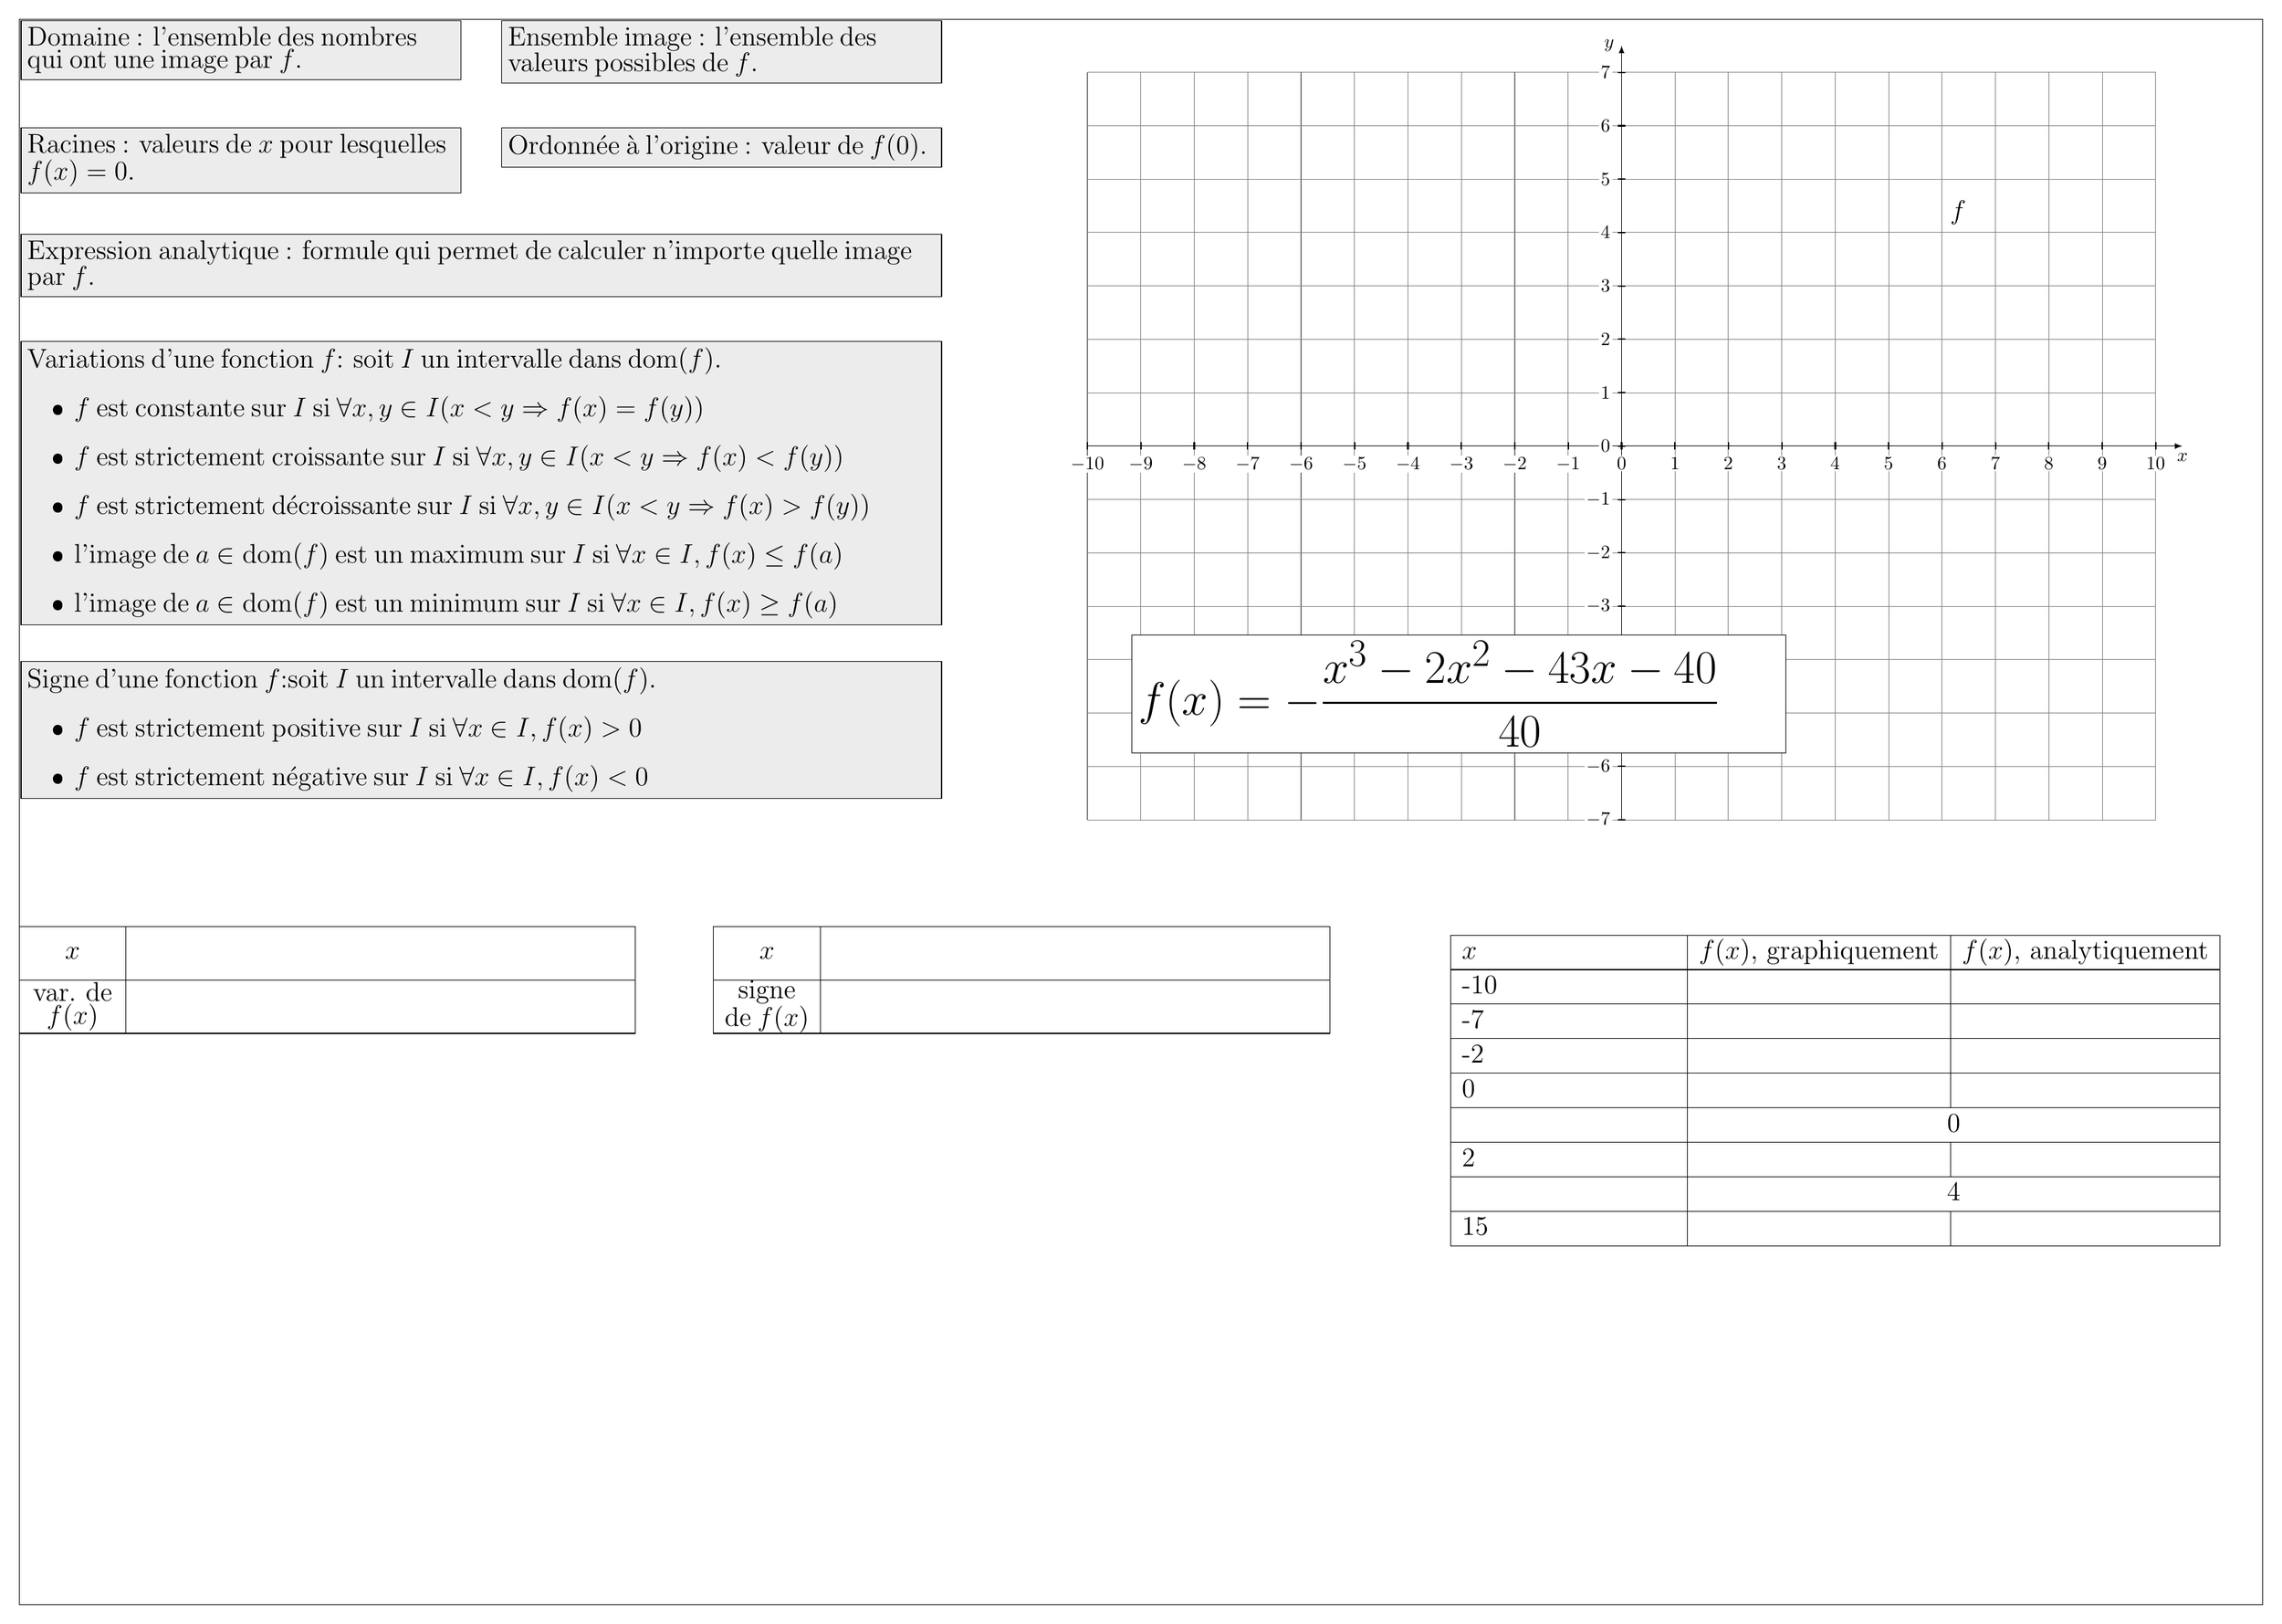
\begin{tikzpicture}

% Définition de la fenêtre du graphique
\tkzInit[xmin=-10,xmax=10,ymin=-7,ymax=7]
\tkzGrid
\tkzAxeXY

% Tracé de la fonction avec les propriétés données
\tkzFct[line width=2pt, domain=-10:10]{((\x + 5)*(\x + 1)*(\x - 8))/(5*1*-8)}
\tkzText[above right](6,4){\Large$f$}
% % Ordonnée à l'origine
% \tkzDefPoint(0,2){A}
% \tkzDrawPoint[color=red](A)
% \tkzLabelPoint[below right, color=red](A){Ordonnée à l'origine $(0,2)$}

% % Racines (aux points -3, 1 et 5)
% \tkzDefPoint(-3,0){B}
% \tkzDefPoint(1,0){C}
% \tkzDefPoint(5,0){D}
% \tkzDrawPoint[color=purple](B)
% \tkzDrawPoint[color=purple](C)
% \tkzDrawPoint[color=purple](D)
% \tkzLabelPoint[below, color=purple](B){Racine}
% \tkzLabelPoint[above, color=purple](C){Racine}
% \tkzLabelPoint[below, color=purple](D){Racine}

% % Points de maximum et minimum locaux (approximations)
% \tkzDefPoint(-5,-4.8){E}
% \tkzDefPoint(8,4.2){F}
% \tkzDrawPoint[color=orange](E)
% \tkzDrawPoint[color=orange](F)
% \tkzLabelPoint[above, color=orange](F){Maximum local $(8, f(8))$}
% \tkzLabelPoint[below, color=orange](E){Minimum local $(-5, f(-5))$}

% Encadrés pour les définitions avec \tkzText

\tkzText[below right,draw, fill=gray!15, text width=8cm](-30,8){\Large
  Domaine : l'ensemble des nombres qui ont une image par $f$.}
\tkzText[below right,draw, fill=gray!15, text width=8cm](-21,8){\Large
  Ensemble image : l'ensemble des valeurs possibles de $f$.}
\tkzText[below right,draw, fill=gray!15, text width=17cm](-30,4){\Large
  Expression analytique : formule qui permet de calculer
  n'importe quelle image par $f$.}

\tkzText[below right,draw, fill=gray!15, text width=8cm](-21,6){\Large Ordonnée à l'origine : valeur de $f(0)$.}
\tkzText[below right,draw, fill=gray!15, text width=8cm](-30,6){\Large Racines : valeurs de $x$ pour lesquelles $f(x) = 0$.}
\tkzText[below right,draw,fill=white, text width=12cm](-9.2,-3.5){\Huge $f(x)=-\dfrac{x^{3}-2x^{2}-43x-40}{40}$
}

\tkzText[below right,draw, fill=gray!15, text width=17cm](-30,2){\Large
  Variations d'une fonction $f$: soit $I$ un intervalle dans $\text{dom}(f)$.
  \begin{itemize}
    \item $f$ est constante sur $I$ si $\forall
      x,y\in I(x<y\Rightarrow f(x)=f(y))$
\item $f$ est strictement croissante sur $I$ si $\forall
  x,y\in I(x<y\Rightarrow f(x)<f(y))$
  \item $f$ est strictement décroissante sur $I$ si $\forall
    x,y\in I(x<y\Rightarrow f(x)>f(y))$
    \item l'image de $a\in\text{dom}(f)$ est un maximum sur $I$ si $\forall x\in
      I, f(x)\le f(a)$
       \item l'image de $a\in\text{dom}(f)$ est un minimum sur $I$ si $\forall x\in
      I, f(x)\ge f(a)$
  \end{itemize}}
\tkzText[below right,draw, fill=gray!15, text width=17cm](-30,-4){\Large Signe d'une fonction $f$:soit $I$ un intervalle dans $\text{dom}(f)$.
  \begin{itemize}
\item $f$ est strictement positive sur $I$ si $\forall
  x\in I, f(x)>0$
  \item $f$ est strictement  négative sur $I$ si $\forall
    x\in I, f(x)<0$
  \end{itemize}}

\tkzDefPoints{12/8/A,-30/-21.7/C}
\tkzText[below ](4,-9){\Large
\begin{tabular}{|p{4cm}|l|l|}
\hline
$x$ & \multicolumn{1}{l|}{$f(x)$, graphiquement} & $f(x)$, analytiquement \\ \hline
-10 & \multicolumn{1}{l|}{}                      &                        \\ \hline
-7  & \multicolumn{1}{l|}{}                      &                        \\ \hline
-2  & \multicolumn{1}{l|}{}                      &                        \\ \hline
0   & \multicolumn{1}{l|}{}                      &                        \\ \hline
    & \multicolumn{2}{c|}{0}                                              \\ \hline
2   & \multicolumn{1}{l|}{}                      &                        \\ \hline
    & \multicolumn{2}{c|}{4}                                              \\ \hline
15  & \multicolumn{1}{l|}{}                      &                        \\ \hline
\end{tabular}
}
\begin{scope}[xshift=-17cm,yshift=-9cm]
\tkzTabInit[espcl=0.3cm]
{\Large$x$
/1,
\Large signe de $f(x)$
/1}
{,}
\end{scope}
\begin{scope}[xshift=-30cm,yshift=-9cm]
\tkzTabInit[espcl=0.3cm]
{\Large$x$
/1,
\Large var. de $f(x)$
/1}
{,}
\end{scope}
\tkzDefRectangle(A,C)\tkzGetPoints{B}{D}
\tkzDrawPolygon(A,...,D)
\end{tikzpicture}

\end{document}